\documentclass{exam}
\usepackage[utf8]{inputenc}
\usepackage{libertine}
\usepackage{graphicx}

\title{\bfseries \sffamily CS 481/681 Computer Graphics Rendering\\Midterm Exam}
\author{%YOURNAMEHERE
}
\date{Due Saturday, March 9th, 2019 9:00am}

\begin{document}

\maketitle

Please answer the questions to the best of your ability. It shouldn't take more than a few sentences per problem. Feel free to use the cited papers for reference.

The following questions refer to this figure.
\begin{figure}[h!]
\centering
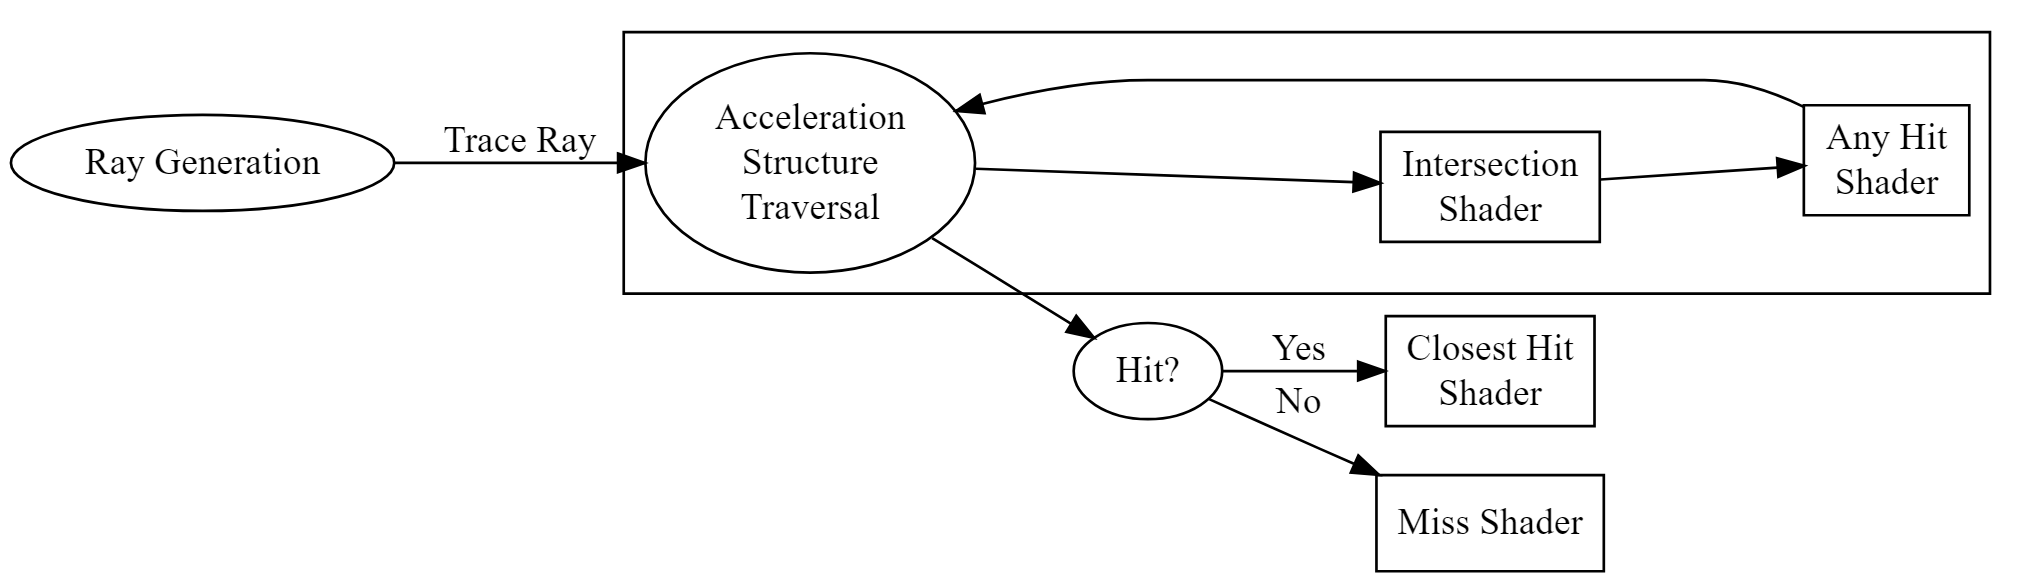
\includegraphics[width=\textwidth]{ray-tracing-pipeline.png}
\caption{Ray Tracing Pipeline\label{fig:pipeline}}
\end{figure}

\begin{questions}

%%-----------------------------------

\question[10] What is the difference between \emph{forward-} and \emph{backward-} ray tracing? How is the ray generation step used to accomplish this step?

\answer % YOUR ANSWER HERE

%%-----------------------------------
\question[10] What is the intersection shader used for? How might sphere tracing~\cite{hart1996sphere} be useful in this context?

\answer % YOUR ANSWER HERE

%%-----------------------------------

\question[10] What is the any hit shader used for? If we wanted to model participating media~\cite{Jarosz:2008:RCP:1330511.1330518} with this shader, we need to understand the difference between the terms homogeneous vs heterogeneous and isotropic vs anisotropic. What is the differences between these terms?

\answer % YOUR ANSWER HERE

%%-----------------------------------

\question[10] After we have determined that we have found no hits while traversing out acceleration structure, we call a miss shader. How might we simulate a physically based sky model~\cite{Hosek:2012:AMF:2185520.2185591}? What factors do we need to consider when using a sky model?

\answer % YOUR ANSWER HERE

%%-----------------------------------

\vspace{2em}
The following questions refer to the rendering equation~\cite{Kajiya:1986:RE:15886.15902}
\begin{equation}
    L_o(\mathbf{x}\to\omega_o) = L_e(\mathbf{x}\to\omega_o) + \int_{\Omega} f_r(\omega_i, \omega_o)\ L_i(\omega_i\to\mathbf{x})\langle \omega_i, \omega_o \rangle\ d\omega_i \,.
\end{equation}

\question[10] The closest hit shader is often used to evaluate the rendering equation. What are the six parts of the rendering equation and what are they used for?

\answer % YOUR ANSWER HERE

%%-----------------------------------

\question[10] For a \emph{bidirectional reflectance distribution function} (BRDF) to be consider physically based~\cite{Heitz2014Microfacet}, it must obey several conditions. Name at least three of them.

\answer % YOUR ANSWER HERE

%%-----------------------------------

\question[10] The specular BRDF introduced by Cook and Torrance~\cite{Cook:1982:RMC:357290.357293} is
\begin{equation}
    f_r(\omega_i, \omega_o) = \frac{f_r(\omega_i, \omega_o) D(\omega_i) G_2(\omega_i)}{4 \cos \theta_i \cos \theta_o}
\end{equation}
What are the functions $f_r(\omega_i, \omega_o)$, $D(\omega)$, and $G_2(\omega_i, \omega_o)$ used for?

\answer % YOUR ANSWER HERE

%%-----------------------------------

\question[10] Distributed ray tracing~\cite{Cook:1984:DRT:964965.808590} allows for a number of special effects. Name at least two and describe how they are used in a production context.

\answer % YOUR ANSWER HERE

%%-----------------------------------

\question[10] Whitted ray tracing~\cite{Whitted:1980:IIM:358876.358882} helped solve what three problems simultaneously in the synthesis of computer generated images?

\answer % YOUR ANSWER HERE

%%-----------------------------------

\question[10] Paul Heckbert~\cite{Heckbert:1990:ART:97880.97895} introduced a regular expression notation for light paths. What rendering method ($\rule{1cm}{0.15mm}$ illumination) is associated with $L\{D|S\}E$ light paths and what rendering method ($\rule{1cm}{0.15mm}$ illumination) is associated with $L\{D|S\}^+E$ light paths.

\answer % YOUR ANSWER HERE

%%-----------------------------------

\end{questions}

\bibliographystyle{alpha}
\bibliography{references}
\end{document}
